%\documentclass[8pt,t,pdflatex,nonotes]{beamer}
%\documentclass[8pt,t,pdflatex,nonotes,aspectratio=169]{beamer}
\documentclass[8pt,t,pdflatex,notes]{beamer}

\usepackage{durham_talk}
\usepackage[english]{babel}
\usepackage{algorithmicx, algpseudocode}
\usepackage{media9}


\setboolean{format169}{false}
\setboolean{insertOutlineSlides}{false}


    
\def\lecturetitle{Performance Assessment and Analysis Guidelines}
\def\brieftitle{Performance Assessment and Analysis} 
\def\session{High-level overview} 
\def\teacher{T.~Weinzierl}
\def\collaborators{T.~Flynn$^\bot$, T.~Weinzierl$^\top$}
\def\affiliation{
 $^\bot$ Advanced Research Computing, Durham University \\
 $^\top$ Institute for Data Science, Computer Science, Durham University
% $^+$ Computer Science, Durham University \\
% $^x$ Computer Science, Technische Universit\"at M\"unchen
} 
\def\date{\today} 


% \title{Task-based implementations of advanced multigrid solvers for Discontinuous Galerkin methods}
% \author[a]{Sean~Baccas}
% \author[b]{Alexander~Belozerov}
% \author[b]{Eike~Hermann~M\"{u}ller}
% \author[c,*]{Tobias~Weinzierl}
% \affil[a]{Advanced Research Computing, Durham University, Durham DH1 3LE, United Kingdom}
% \affil[b]{Department of Mathematical Sciences, University of Bath, Bath BA2 7AY, Bath, United Kingdom}
% \affil[c]{Department of Computer Science, Durham University, Durham DH1 3LE, United Kingdom}
% \affil[*]{Email: \texttt{tobias.weinzierl@durham.ac.uk}}


\begin{document}

%\includeversion{notes}
\excludeversion{notes}
 
 


\begin{frame}
 \titlepage
\end{frame}


\begin{frame}
 \frametitle{Acknowledgements}
 \begin{center}
   
\includegraphics[width=0.3\textwidth]{logos/ukri.png}
 \end{center}
 \vfill
This work was supported by the Engineering and Physical Sciences Research Council [grant number XXXX]. The underlying project SHAREing (Skills Hub for Accelerated Research Environments Inspiring the Next Generation) is part of the cross-UKRI Digital Research Infrastructure initiative.

\vspace{0.2cm}

This work was also supported by the Science and Technology Facilities Council [grant number UKRI/ST/B000293/1]. The underlying project HAI-End is part of the cross-UKRI Digital Research Infrastructure initiative.
 \vfill
\end{frame}


\begin{frame}
  \frametitle{Disclaimer}
  \vfill
  There is no right or wrong or unique approach{\footnotesize $^*$}. 
  \vfill
  {\footnotesize $^*$ but there is material that we collect on our Sharepoint site.}
\end{frame}


\begin{frame}
  \frametitle{Prepare a benchmark}
  \vfill
  \begin{itemize}
    \item No user interaction.
    \item Easy to scale that benchmark up and down, i.e.~to make the problem solved slightly bigger or smaller. 
    \item Representative of a real-world run.
    \item 3--5 minutes.
    \item The benchmark has to represent performance characteristics.
  \end{itemize}
  \pause
  \begin{itemize}
    \item No I/O (unless you benchmark I/O).
    \item Focus on single-node run.
    \item Memory footprint bigger than L3 cache (60--80\% of main memory).
    \item A test node should be a node similar to the production runs machine
    \item Node should be accessed exclusively
  \end{itemize}
  \vfill
\end{frame}


\begin{frame}
  \frametitle{Understanding code}
  \vfill
  When we alter problem sizes, we have to be sure we compare the right things.
  \begin{itemize}
    \item Computational complexity $\mathcal{O}(N^p)$
    \item Often favourable to work with normalised time $T^{(0)}(t)$
    \item Suggestion: Run a few experiments and calibrate your normalisation function
  \end{itemize}
  \vfill
\end{frame}


\begin{frame}
 \frametitle{High-level rubrics}
 \vfill
 \begin{center}
   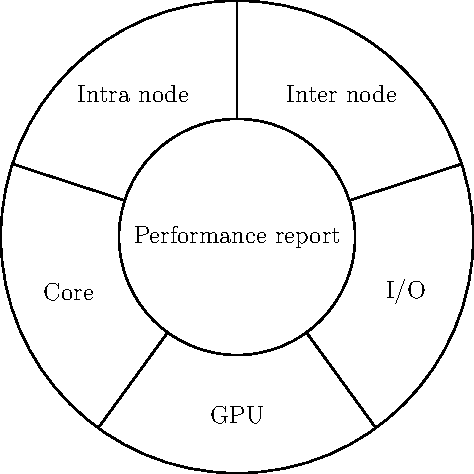
\includegraphics[width=0.6\textwidth]{../high-level/performance_diag.pdf}
 \end{center}
 \vfill
\end{frame}


\begin{frame}
 \frametitle{Core-level: objective}
 \vfill
 \begin{citation-box}{QoI}
   For the core-level analysis, we examine how efficiently your code harnesses the chip's microarchitecture. 
   \begin{itemize}
     \item Does your code leverage the most advanced instruction sets available? 
     \item Does it properly utilise the memory interconnect? 
   \end{itemize}
 \end{citation-box}
 \begin{center}
   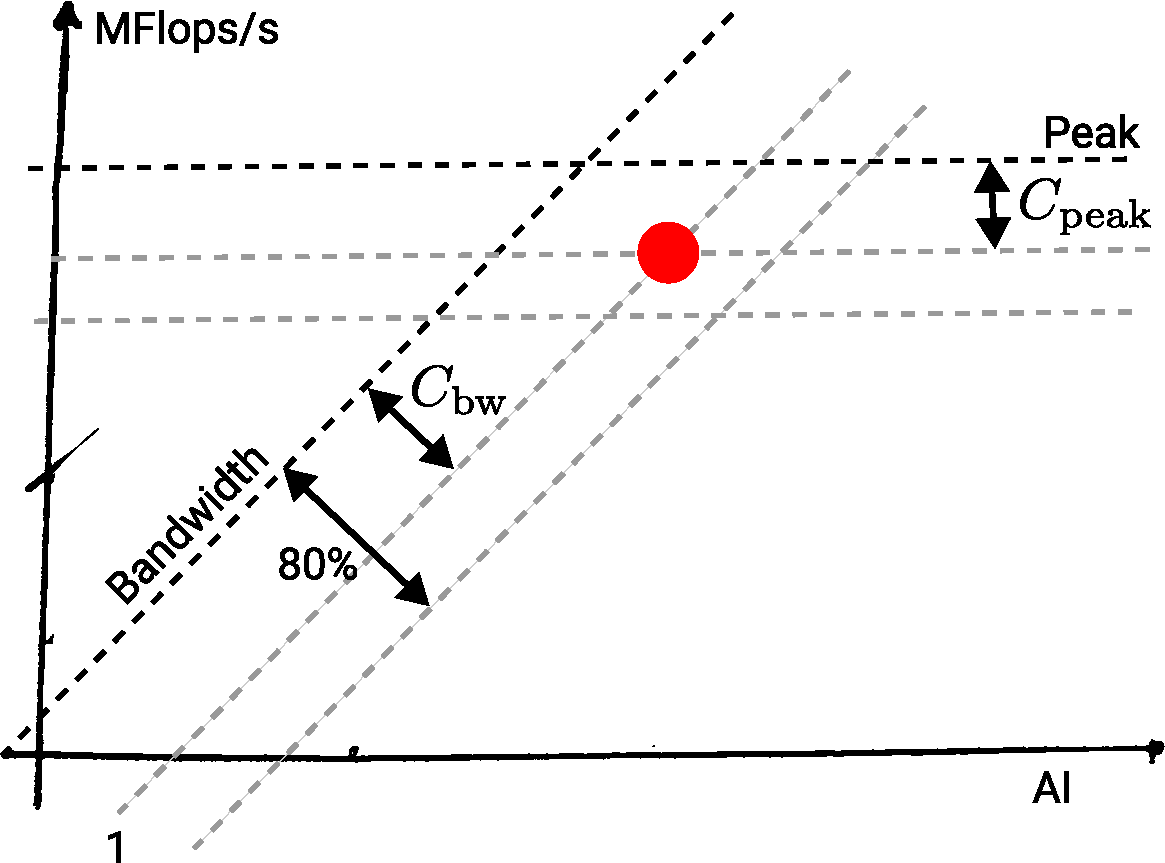
\includegraphics[width=0.6\textwidth]{../high-level/core-architecture.pdf}
 \end{center}
 \vfill
\end{frame}


\begin{frame}[fragile]
 \frametitle{Core-level: Roofline model}
 \vfill
 \begin{center}
   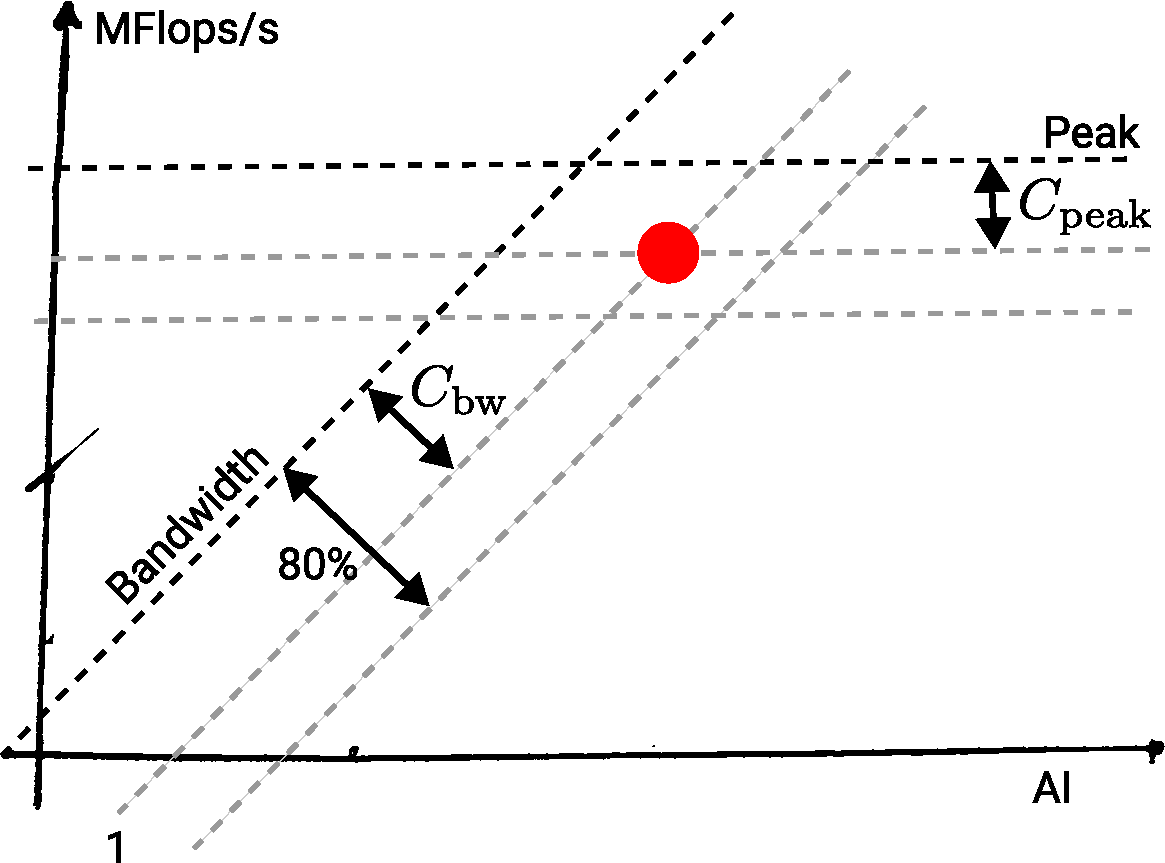
\includegraphics[width=0.6\textwidth]{../high-level/core-architecture.pdf}
 \end{center}
\begin{verbatim}
likwid-bench -t triad -W S0:2GB:1
likwid-bench -t triad -W N:2GB:128
likwid-bench -t peakflops -w S0:10000MB:1
\end{verbatim}
 \begin{itemize}
   \item Peak on one core sufficient
   \item Max memory bandwidth either on core or node 
 \end{itemize}
 \vfill
\end{frame}


\begin{frame}[fragile]
 \frametitle{Core-level: Code characterisation}
 \vfill
 \begin{center}
   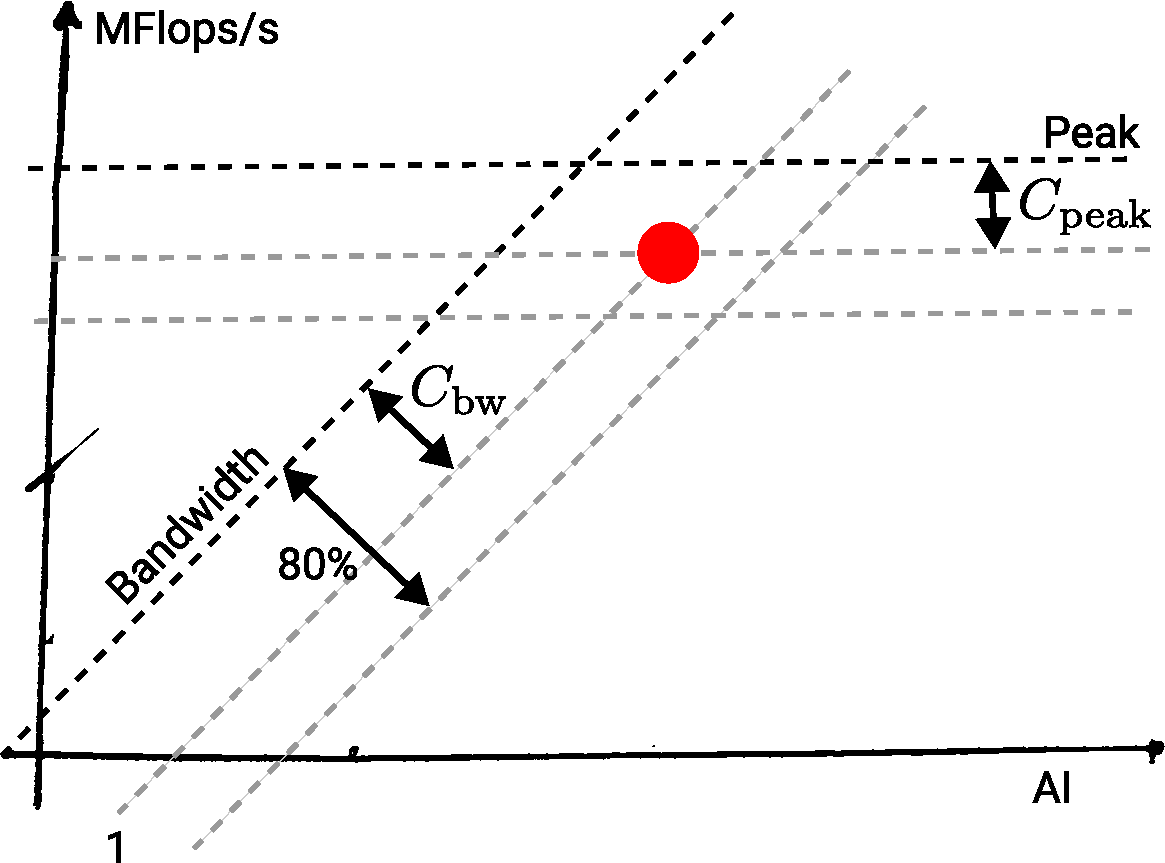
\includegraphics[width=0.6\textwidth]{../high-level/core-architecture.pdf}
 \end{center}
\begin{verbatim}
likwid-perfctr -f -C 0 -g MEM ./mycode
likwid-perfctr -f -C 0 -g FLOPS_DP ./mycode
\end{verbatim}
 \begin{itemize}
   \item Identify red dot and fractions $C_{\text{bw}}$ and $C_{\text{peak}}$
   \item Other tools provide similar data (e.g., Linaro and Intel)
 \end{itemize}
 \vfill
\end{frame}


\begin{frame}[fragile]
 \frametitle{Core-level: Evaluation}
 \vfill
\begin{center}
 \begin{tabular}{r|p{0.22\textwidth}p{0.22\textwidth}p{0.22\textwidth}}
  & $C_{\text{bw}}\geq 0.8$ & $0.8 > C_{\text{bw}}\geq 0.6$ & $0.6 > C_{\text{bw}}$ \\
  \hline
  $f_{\text{peak}} \geq 0.8$
   & \cellcolor{green!25}
   & \cellcolor{green!25} perfect
   & \cellcolor{orange!25}
  \\
  $0.8 > f_{\text{peak}} \geq 0.6$
   & \cellcolor{green!25}
   & \cellcolor{orange!25} 
   & \cellcolor{orange!25} flaw
  \\
  $0.6 > f_{\text{peak}}$
   & \cellcolor{red!25}
   & \cellcolor{red!25} severe flaw
   & \cellcolor{red!25} 
 \end{tabular}
\end{center}

%{equation:intra-node:performance-model}

\begin{citation-box}{Compute-bound regime}
 If $f_{\text{peak}} \geq 0.8$, the code does uses the compute capabilities (very) efficiently.
 However, if the bandwidth $C_{\text{bw}}< 0.6$, there might still be additional space to improve the throughput and to speed up the code. 
\end{citation-box}


\begin{citation-box}{Not compute-bound and maybe not even memory-bound}
 If $0.6 \leq f_{\text{peak}}< 0.8$, the code does not use the compute units particularly efficiently and we have to investigate further.
 However, if $f_{\text{bw}} \geq 0.8$, the problem might be inherently memory-bound (to be checked), in which case there might be limited potential to optimise further.
\end{citation-box}
 \vfill
\end{frame}


\begin{frame}
  \frametitle{Intra-node: objective}
  \vfill
  \begin{citation-box}{QoI}
   Do we use all the hardware threads efficiently?
  \end{citation-box}
  \begin{center}
    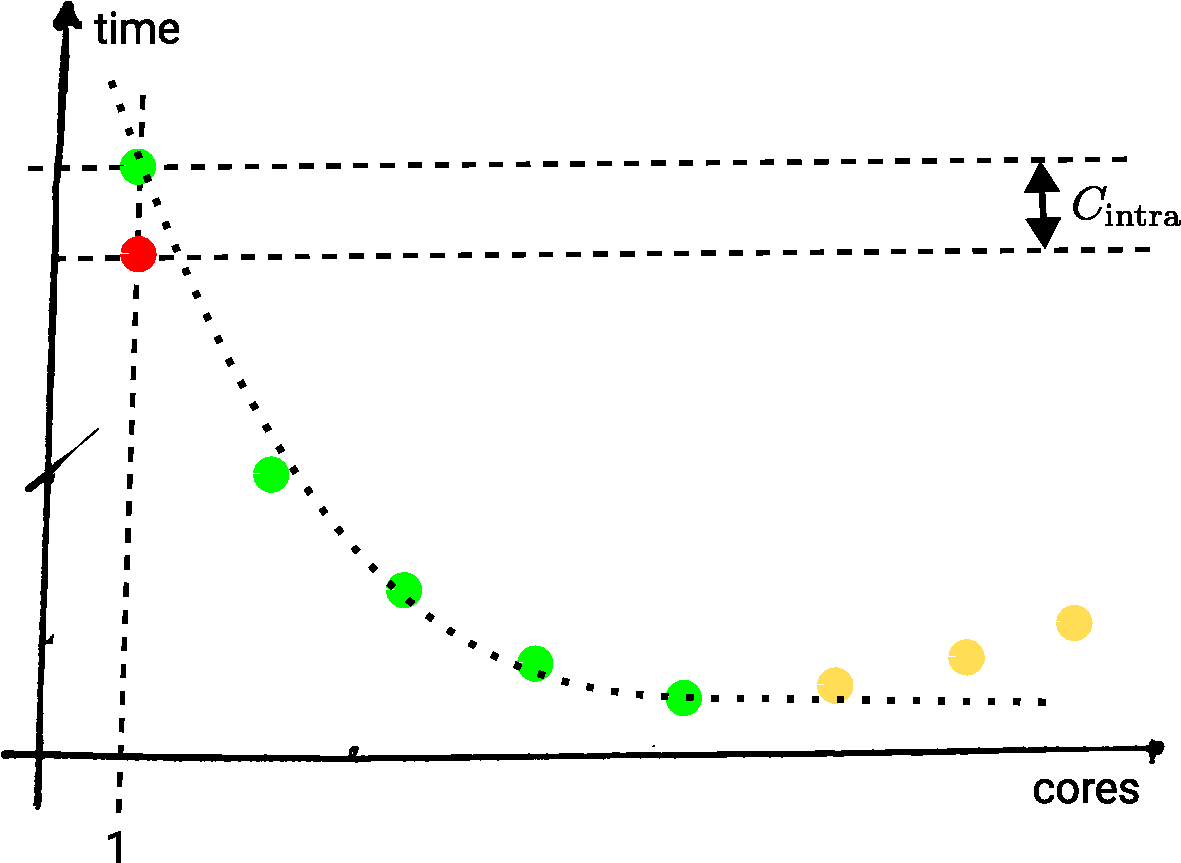
\includegraphics[width=0.7\textwidth]{../high-level/intra-node.pdf}
  \end{center}
  \vfill
\end{frame}


\begin{frame}
  \frametitle{Intra-node: strong scaling}
  \vfill
  \begin{center}
    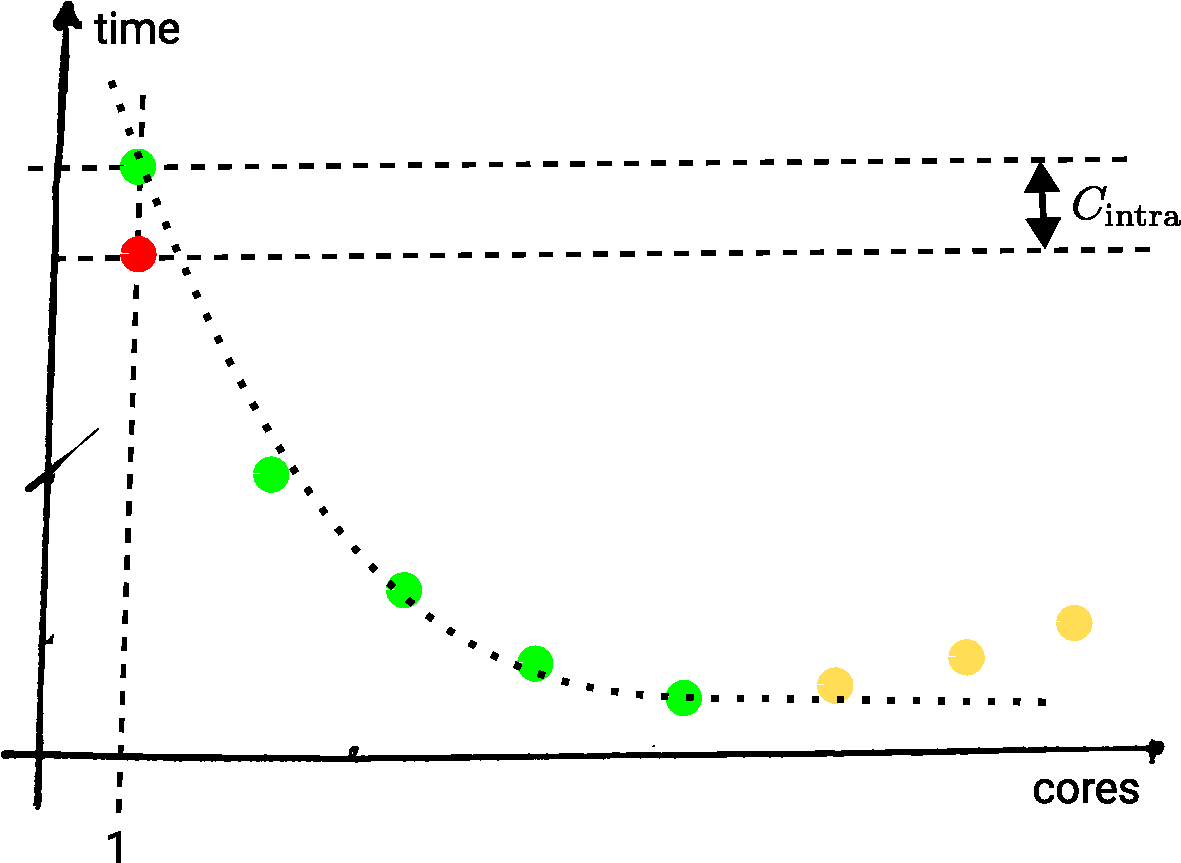
\includegraphics[width=0.6\textwidth]{../high-level/intra-node.pdf}
  \end{center}
\[
 t(p_{\text{threads}}) = \frac{t_{\text{serial}}}{C_{\text{intra}}}\left( f_{\text{intra}}/p_{\text{threads}} + (1-f_{\text{intra}}) \right).
\]
  \begin{itemize}
    \item Amdahl's law plus calibration term $C_{\text{intra}}$
    \item Assessment evaluates $C_{\text{intra}}$ and $f_{\text{intra}}$
  \end{itemize}
  \vfill
\end{frame}


\begin{frame}[fragile]
  \frametitle{Intra-node: data collection}
  \vfill
\[
 t(p_{\text{threads}}) = \frac{t_{\text{serial}}}{C_{\text{intra}}}\left( f_{\text{intra}}/p_{\text{threads}} + (1-f_{\text{intra}}) \right).
\]
  \begin{itemize}
    \item $t_{\text{serial}}$ and $t(1)$ $\Rightarrow \ C_{\text{intra}}$
    \item Measure different core/thread counts:
    \begin{itemize}
      \item OpenMP: \texttt{export OMP\_NUM\_THREADS=xxx}
      \item Slurm settings
      \item Manual taskset:
      \begin{verbatim}
taskset -c 0-3 ./myexec
\end{verbatim}
    \end{itemize} 
    \item Regression/parameter fitting
  \end{itemize}
  \vfill
\end{frame}


\begin{frame}
  \frametitle{Intra-node: Evaluation}
  \vfill
\begin{center}
 \begin{tabular}{r|p{0.22\textwidth}p{0.22\textwidth}p{0.22\textwidth}}
  & $C_{\text{intra}}\geq 0.8$ & $0.8 > C_{\text{intra}}\geq 0.6$ & $0.6 > C_{\text{intra}}$ \\
  \hline
  $f_{\text{intra}} \geq 0.8$
   & \cellcolor{green!25} perfect
   & \cellcolor{orange!25}
   & \cellcolor{red!25}
  \\
  $0.8 > f_{\text{intra}} \geq 0.6$
   & \cellcolor{orange!25}
   & \cellcolor{orange!25} flaw
   & \cellcolor{red!25}
  \\
  $0.6 > f_{\text{intra}}$
   & \cellcolor{red!25}
   & \cellcolor{red!25}
   & \cellcolor{red!25} severe flaw
 \end{tabular}
\end{center}
\begin{citation-box}{Overheads}
 If $C_{\text{intra}}< 0.8$, the implementation introduces a significant overhead for the multithreading.
 If $C_{\text{intra}}< 0.6$, the overhead is severe.
\end{citation-box}


\begin{citation-box}{Scalability}
 If $f_{\text{intra}}< 0.8$, the code does not scale particularly well over the threads.
 If $f_{\text{intra}}< 0.6$, the scaling is severely poor.
\end{citation-box}
  \vfill
\end{frame}


\begin{frame}
 \frametitle{Partners}
 \vfill
 % Supported by DiRAC
 % Supported by CS in Duram University Proud member of VI-HPS
 \vfill
\end{frame}


\end{document}
